\documentclass[10pt]{article}
\usepackage[letterpaper,margin=1in]{geometry}
\usepackage{times}
\renewcommand{\ttdefault}{cmtt}
\usepackage{amsmath,amssymb}
\usepackage{booktabs,tabularx,array}
\usepackage{graphicx}
\usepackage[font=small,labelfont=bf]{caption}
\usepackage{enumitem}
\usepackage[numbers,sort&compress]{natbib}
\usepackage[hidelinks]{hyperref}
\usepackage{float}
\usepackage{tikz}
\usetikzlibrary{positioning,arrows.meta}
\setlist{nosep,leftmargin=1.4em}
\setlength{\parskip}{0.35em}
\setlength{\parindent}{0pt}
\renewcommand{\arraystretch}{1.12}

\title{\textbf{Position and Format Bias in Qwen3 Judges Across Model Scale and Thinking Mode}\\[0.3em]
\large DSC 261 Midterm Report (Group 3)}
\author{Pradyumna Sripada \quad Chinmay Nadgir \quad Krishna Kanth Kodanganti\\
Shashank Reddyhalli Rakesh \quad Akbota Assan (Lily)\\
\small UC San Diego, Hal\i c\i o\u{g}lu Data Science Institute}
\date{November 2026}

\begin{document}
\maketitle

\begin{abstract}
LLM judges rank models and select training data. A verdict that depends on how answers are presented rather than
on what they say is therefore a validity failure. We test for this with \emph{content-preserving} edits to Chatbot
Arena answer pairs. We either swap the order of the two answers (position) or delete their markdown headings, bold
and bullet markers while keeping every word (format). We then subtract a \emph{noise floor} measured by judging
identical inputs twice. This midterm applies the complete per-pair design (10 judge calls per pair) to a frozen
100-pair subset, which is 10\% of the planned sample. We run Qwen3 judges at 0.6B, 1.7B, 4B and 8B parameters with
thinking off and on: 8 configurations, 8{,}000 calls, 0 invalid verdicts.
\begin{itemize}
\item \textbf{Position.} Order changes verdicts far beyond noise. The excess flip rate is 15--73.5 percentage
points in seven of eight configurations. For the pre-registered test configuration (8B with thinking) it is 15.0
points, 95\% CI 5.0--25.5, above the 2-point threshold.
\item \textbf{Thinking.} Thinking mode lowers the excess by 30.5 points on average (18.3 points excluding 0.6B).
Part of this may come from the different sampling settings each mode uses; the planned check that separates
the two has not yet been run.
\item \textbf{Format.} Removing markdown rarely changes the winning answer beyond noise. When exactly one answer
keeps its markdown, four of eight configurations (1.7B and 8B with thinking off, 4B in both modes) choose it in
53.5--58\% of verdicts, significantly above 50\% after Holm correction. The others stay within 50.5--52.2\%.
\item \textbf{Human agreement.} Agreement with human voters (51--66\%, about $\pm$10 points at $n=100$) is close
to a length-only baseline (57\%).
\end{itemize}
The 4B and 8B judges are quantized, so differences between sizes are confounded with numerical precision.
\end{abstract}

\section{Introduction}
Pairwise LLM judges read a question and two answers and return a preference. They now sit inside benchmarks,
model selection and reinforcement-learning pipelines \citep{zheng2023judging}. If the verdict tracks a surface
feature such as answer order or formatting, developers who rely on it are misled. Optimizers that select against
it can also exploit the feature without improving content \citep{zhang2025lists,gao2023scaling,zhou2026selfplay}.

\subsection{Research questions and hypotheses}
These hypotheses are taken from our proposal; their thresholds were fixed before any judge was run.
\begin{itemize}
\item \textbf{RQ1 / H1 (existence).} For position and for format, the largest judge with thinking on has an
\emph{excess flip rate} (flip rate under the edit minus the noise floor) whose 95\% CI lower bound exceeds
2 percentage points.
\item \textbf{RQ2 / H2 (size and thinking).} The excess flip rate changes with model size (per doubling) and with
thinking mode. The smallest effect of interest is 3 points, and the test runs in both directions, so H2 can also
fail by showing the effects are negligible.
\item \textbf{RQ3 / H3 (cost under selection).} Under best-of-4 selection, the judge's pick contains markdown
more often than the gold-proxy pick does. The gold proxy is the mean of UltraFeedback's four
fine-grained GPT-4 ratings \citep{cui2024ultrafeedback}.
\end{itemize}
This midterm reports RQ1 and RQ2 on a 100-pair subset. RQ3 is scheduled for the second half (Section~\ref{sec:plan}).

\textbf{Contributions so far.}
\begin{enumerate}
\item A frozen, reproducible data pipeline over 168{,}634 Chatbot Arena conversations, with every filter step
counted (Table~\ref{tab:filters}).
\item A deterministic markdown stripper with an automatic word-sequence check (2{,}400 of 2{,}400 answers pass)
and a 50-pair audit (AI first pass; team sign-off pending).
\item A judge harness that renders Qwen3's own chat template, enforces a 2{,}048-token thinking budget and resumes
after crashes. With it we ran the full 10-call design for 8 configurations (Figure~\ref{fig:pipeline}).
\item Interim estimates of position and format bias with noise-floor correction and bootstrap CIs, a GEE model of
the size and thinking effects, and robustness checks.
\end{enumerate}

\begin{figure}[H]
\centering\small
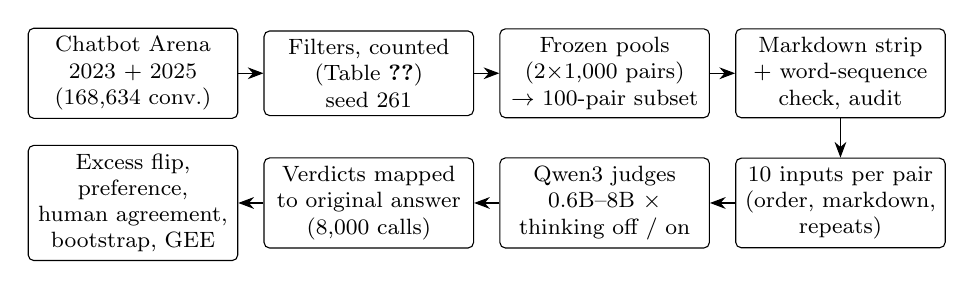
\begin{tikzpicture}[node distance=0.32cm and 0.32cm, box/.style={draw, rounded corners=2pt, align=center,
  inner sep=3pt, text width=2.45cm, font=\footnotesize}, >={Stealth[length=2mm]}]
\node[box] (a) {Chatbot Arena\\2023 + 2025\\(168{,}634 conv.)};
\node[box, right=of a] (b) {Filters, counted\\(Table~\ref{tab:filters})\\seed 261};
\node[box, right=of b] (c) {Frozen pools\\(2$\times$1{,}000 pairs)\\$\rightarrow$ 100-pair subset};
\node[box, right=of c] (d) {Markdown strip\\+ word-sequence\\check, audit};
\node[box, below=0.5cm of d] (e) {10 inputs per pair\\(order, markdown,\\repeats)};
\node[box, left=of e] (f) {Qwen3 judges\\0.6B--8B $\times$\\thinking off / on};
\node[box, left=of f] (g) {Verdicts mapped\\to original answer\\(8{,}000 calls)};
\node[box, left=of g] (h) {Excess flip, preference,\\human agreement,\\bootstrap, GEE};
\draw[->] (a)--(b); \draw[->] (b)--(c); \draw[->] (c)--(d); \draw[->] (d)--(e);
\draw[->] (e)--(f); \draw[->] (f)--(g); \draw[->] (g)--(h);
\end{tikzpicture}
\caption{Pipeline of the midterm study. Every stage is a script or notebook; outputs are hashed and logged.}
\label{fig:pipeline}
\end{figure}

\section{Related Work}
\citet{zheng2023judging} introduced MT-Bench and Chatbot Arena and documented position, verbosity and
self-enhancement bias in LLM judges. \citet{zhang2025lists} showed that reward models and GPT-4 favour lists, bold
text and links, and that best-of-$n$ selection and online DPO exploit this preference. \citet{soumik2026judging}
compared nine debiasing strategies across five judges and found style bias (markdown over prose) to be far larger
than position bias. Our preliminary results on small Qwen3 judges show the opposite ordering, a contrast we
return to in Section~\ref{sec:disc}. \citet{zhou2026taxonomic} injected 12 biases by controlled rewriting and
trained debiased judges. \citet{huang2026reasoning} and \citet{wang2025assessing} found that reasoning judges are
more accurate but retain position and superficial-quality biases. \citet{jayarao2025explicit} reported that
thinking Qwen3 judges (0.6B--4B) are more consistent. \citet{yang2026auditing} audited Qwen3 judges from 1.7B to
32B and found that size reduces but does not remove position and verbosity bias. \citet{gao2023scaling} and
\citet{zhou2026selfplay} studied optimization against imperfect reward models and judges. Our design differs in
combining content-preserving edits with a measured noise floor, toggling thinking on identical weights, and (in
the final report) linking each judge's measured bias to its best-of-$n$ selections.

\section{Data}
\label{sec:data}
\textbf{Sources.} The main pool is the 2023 Chatbot Arena human-preference release, with 33{,}000
conversations.\footnote{Loaded from a structurally identical public mirror (revision \texttt{d45bf83}) of the gated
repository \url{lmsys/chatbot_arena_conversations}. A re-run on the official file is pending.} The supplement is
the 2025 Arena release, with 135{,}634 conversations under CC-BY-4.0.\footnote{\url{lmarena-ai/arena-human-preference-140k},
revision \texttt{6322995}.} MT-Bench expert votes and UltraFeedback are prepared (1{,}284 votes; 500 prompts
with 4 answers each) for the second half.

\textbf{Filters.} We keep English, single-turn, text-only pairs with a non-tied human vote. Answer lengths, counted
in words with markdown markers excluded, must differ by at most a factor of 2. Answers with tables or code blocks
are excluded, because stripping them would change content. Table~\ref{tab:filters} gives the counts. Only 170
pairs from 2023 have markdown in \emph{both} answers. As pre-registered, the format pool is therefore filled with
2025 pairs under the same filters and labelled by source.

\begin{table}[H]
\centering\small
\caption{Filtering of the Chatbot Arena releases (pairs remaining after each step).}
\label{tab:filters}
\begin{tabular}{lrr}
\toprule
Step & 2023 release & 2025 release \\
\midrule
Loaded & 33{,}000 & 135{,}634 \\
English (dataset label) & 29{,}206 & 71{,}175 \\
Single turn, text only, non-empty & 25{,}904 & 60{,}895 \\
Non-tied human vote & 18{,}296 & 44{,}299 \\
Answers differ; $\geq$95\% Latin script in prompt and both answers & 18{,}138 & 43{,}089 \\
Both answers non-empty after marker removal; length ratio $\leq 2$ & 9{,}463 & 25{,}567 \\
No tables or code blocks & 8{,}327 & 16{,}141 \\
Exact duplicates removed; judge prompt $\leq$ 6{,}000 tokens & 8{,}325 & 16{,}052 \\
\midrule
Markdown in both answers (before / after strip check) & 170 / 169 & 11{,}461 / 11{,}308 \\
\bottomrule
\end{tabular}
\end{table}

\textbf{Pools and midterm subset.} We froze three sets with seed 261, keeping one pair per prompt: a
1{,}000-pair position pool (2023), a 1{,}000-pair format pool (167 pairs from 2023 and 833 from 2025), and
reserves (200 position, 198 format). One pair per prompt removes 2 of the 169 eligible 2023 format pairs,
leaving 167. File hashes are recorded in a manifest. The \textbf{midterm subset} is
100 pairs drawn from the format pool: 84 from 2025 and 16 from 2023. Both answers in every pair contain markdown,
so the same pairs support the position and the format tests. Position bias in this midterm is therefore measured
on markdown-heavy, mostly 2025 pairs, not on the 2023 position pool. Answers have a median length of 380 words
(range 65--2{,}077). The judge prompt averages 1{,}813 tokens (maximum 5{,}917). Voters preferred answer A in 45
of the 100 pairs.

\textbf{Markdown edit.} The ``plain'' variant removes ATX headings (lines starting with \texttt{\#}),
\texttt{**bold**} markers and line-initial bullet markers (\texttt{-}, \texttt{*}, \texttt{+}). Line breaks are
kept, so list items stay on separate lines. Italics and numbered lists are left unchanged. An independent check
confirms that the words and their order are identical before and after stripping. On the frozen pools,
2{,}400 of 2{,}400 answers pass, and 160 candidate answers that failed were excluded before freezing.

\textbf{Audit.} We audited 50 pairs (100 answers). The first pass was done by an AI reviewer working through a
checklist, with sign-off by team members still pending. It found meaning and wording preserved in all 100 answers.
Two answers with three-level nested lists became hard to read, and their pairs were replaced in the format pool.
These two pairs remain in the midterm subset, which was drawn before the audit. Excluding them changes no position or
format excess flip rate by more than 1.3 points (Appendix~\ref{app:robust}).

\textbf{Human preference for markdown.} Across all eligible pairs where exactly one answer uses markdown, voters
chose the markdown answer 56.9\% of the time in 2023 (95\% CI 53.5--60.1, $n=853$) and 56.3\% in 2025
(54.5--58.1, $n=2{,}829$). The effect survives control for length: a logistic regression with prompt-clustered
standard errors gives odds ratios of 1.21 and 1.15, $p \leq 0.009$. Human labels therefore carry some format
preference themselves.

\section{Method}
\subsection{Judges}
We use the original hybrid Qwen3 checkpoints \citep{qwen2025qwen3}, which support both modes in one model
(not the later separate Instruct and Thinking releases), pinned to their Hugging Face
revisions (Table~\ref{tab:judges}). Thinking is switched with the chat template's \texttt{enable\_thinking}
flag on identical weights. With thinking off, the template pre-fills an empty \texttt{<think></think>} block, so
reasoning is disabled rather than hidden. Hardware limited the two larger models: 4B was quantized to 8 bits by
us, and 8B uses Qwen's official 4-bit AWQ (activation-aware weight quantization) build \citep{lin2024awq}. Our evaluation contract (the list of settings and analyses we froze before running any
judge) specifies 16-bit weights for all sizes, so this is a deviation, and every configuration is reported separately.

\begin{table}[H]
\centering\small
\caption{Judge configurations. Each size runs with thinking off and on. MLX is Apple's on-device inference
library; vLLM is a GPU inference server.}
\label{tab:judges}
\begin{tabular}{llll}
\toprule
Size & Checkpoint (revision) & Weights & Backend, hardware \\
\midrule
0.6B & \texttt{Qwen/Qwen3-0.6B} (\texttt{c1899de}) & BF16 & MLX, Apple M2 Pro (16\,GB) \\
1.7B & \texttt{Qwen/Qwen3-1.7B} (\texttt{70d244c}) & BF16 & MLX, Apple M2 Pro \\
4B & \texttt{Qwen/Qwen3-4B} (\texttt{1cfa9a7}) & 8-bit, group 64 & MLX, Apple M2 Pro \\
8B & \texttt{Qwen/Qwen3-8B-AWQ} (\texttt{4da05a8}) & 4-bit AWQ & vLLM 0.8.5, RTX 3070 Laptop (8\,GB) \\
\bottomrule
\end{tabular}
\end{table}

\textbf{Prompt and decoding.} The judge receives the MT-Bench pairwise prompt (``pair-v2''
\citep{zheng2023judging}) with the tie option removed, since our pools contain no ties. It must end with
\texttt{[[A]]} or \texttt{[[B]]}. Sampling follows each mode's model-card settings \citep{qwen2025qwen3}:
\begin{itemize}
\item Thinking on: temperature 0.6, top-$p$ 0.95, top-$k$ 20.
\item Thinking off: temperature 0.7, top-$p$ 0.8, top-$k$ 20.
\end{itemize}
The two modes therefore also differ in sampling. Section~\ref{sec:h2} reports a check that separates the two.
Thinking is capped at 2{,}048 tokens. On truncation we close the reasoning block with Qwen's early-stop sentence
and allow 512 more tokens for the verdict. The verdict is the last \texttt{[[A]]} or \texttt{[[B]]} after the
reasoning block. An unparseable output gets one retry with a fresh seed, and is otherwise counted as invalid and
as a flip. Each request has its own seed. Part of the 1.7B--4B run used batched generation, where the seed is set
per batch; repeated inputs still never share a sampling stream.

\subsection{Design: ten judge calls per pair}
For a pair with answers $a$ and $b$, each with a markdown version $m$ and a plain version $p$, every configuration
judges the ten inputs in Table~\ref{tab:design}. Each verdict is mapped back to the original answer that won.

\begin{table}[H]
\centering\small
\caption{The ten judge calls per pair and configuration. The two all-plain calls are collected for the full
study's $2\times2$ analysis but are not used by the measures in this report.}
\label{tab:design}
\begin{tabular}{lll}
\toprule
Calls & Inputs (shown first, shown second) & Purpose \\
\midrule
2 & $(a^m, b^m)$, $(b^m, a^m)$ & position: original vs.\ swapped order \\
2 & $(a^m, b^m)$, $(b^m, a^m)$, repeated & noise floor: identical input judged again \\
4 & $(a^p,b^m)$, $(a^m,b^p)$ in both orders & format: exactly one answer stripped \\
2 & $(a^p,b^p)$ in both orders & both stripped (not used here) \\
\bottomrule
\end{tabular}
\end{table}

\subsection{Measures}
Let $w(\cdot)$ denote the winning original answer for an input.
\begin{itemize}
\item \textbf{Position flip rate}: the share of pairs with $w(a^m,b^m) \neq w(b^m,a^m)$.
\item \textbf{Noise floor}: the share of disagreements between two runs on the same input, averaged over both orders.
\item \textbf{Excess flip rate} (main measure): flip rate minus noise floor, in percentage points. It isolates the
effect of the edit from sampling randomness.
\item \textbf{Format flip rate}: the share of the four one-stripped inputs whose winner differs from the
all-markdown input in the same order.
\item \textbf{First-slot preference}: the share of verdicts for the answer shown first. 50\% means no lean.
\item \textbf{Markdown preference}: across the one-stripped inputs, the share of verdicts for the answer that
kept its markdown. Because each order contributes one input where $a$ is stripped and one where $b$ is stripped,
content and position effects cancel, so 50\% is the exact null.
\item \textbf{Human agreement}: accuracy and Cohen's $\kappa$ of the original-order verdict against the Arena
vote. \emph{Swap-and-average} agreement gives 0.5 credit to a pair whose verdict flips with order.
\end{itemize}

\textbf{Why two format measures.} The format excess flip rate cannot detect a consistent preference for
markdown. Stripping the baseline \emph{winner} tends to flip the verdict; stripping the baseline \emph{loser}
tends to entrench it. These two effects cancel in the average. For example, for 4B with thinking, stripping the
winner flips 22\% of verdicts and stripping the loser flips 6\% (Appendix~\ref{app:robust}). We therefore report
markdown preference as the direct test of format bias. The format excess flip rate is kept because it is the
pre-registered H1 measure.

\textbf{Statistics.} We use 95\% percentile bootstrap intervals over pairs (10{,}000 resamples, seed 261). Each
pair is its own prompt cluster. Per-configuration intervals are unadjusted. Bonferroni-adjusted bounds for 8
configurations are given in Appendix~\ref{app:robust}. Markdown preference is tested against 50\% with Holm
correction across the 8 configurations. Human-agreement accuracies are reported with Wilson intervals.

For RQ2 we fit a GEE (generalized estimating equations) logistic regression with exchangeable within-pair
correlation:
\[\text{flip} \sim \text{edit} \times (\log_2 \text{size} + \text{thinking}).\]
Here \emph{edit} is 1 for an order swap and 0 for a repeat, and size is in billions of parameters. The
edit$\times$size and edit$\times$thinking terms measure how the excess flip rate changes. We convert them to
average marginal effects (AMEs) in percentage points and attach cluster-bootstrap intervals (300 refits,
independence working correlation, for runtime). This is a reduced form of the pre-registered model: it covers
position only and omits the three-way size$\times$thinking term (Section~\ref{sec:plan}). The pre-registered
equivalence test for H2 (two one-sided tests against $\pm$3 points) is deferred to the full sample; here we report
the AME intervals only.

\section{Results}
\subsection{Run statistics}
All 8{,}000 judge calls returned a parseable verdict on the first attempt (Table~\ref{tab:runs}). Between 0.6\%
and 1.2\% of thinking runs reached the 2{,}048-token budget. Thinking multiplies output length by 2.8--4.2.

\begin{table}[H]
\centering\small
\caption{Run statistics per configuration (1{,}000 calls each; no invalid verdicts and no retries anywhere).}
\label{tab:runs}
\begin{tabular}{lrrr}
\toprule
Configuration & Truncated (of 1{,}000) & Mean output tokens & Mean thinking tokens \\
\midrule
0.6B, thinking off & -- & 105 & -- \\
0.6B, thinking on & 6 & 440 & 366 \\
1.7B, thinking off & -- & 175 & -- \\
1.7B, thinking on & 12 & 567 & 477 \\
4B (8-bit), thinking off & -- & 220 & -- \\
4B (8-bit), thinking on & 9 & 612 & 566 \\
8B (4-bit), thinking off & -- & 203 & -- \\
8B (4-bit), thinking on & 7 & 624 & 592 \\
\bottomrule
\end{tabular}
\end{table}

\subsection{Position bias (RQ1)}
Table~\ref{tab:main} and Figure~\ref{fig:excess}a show that swapping answer order changes the verdict far more
often than repeated sampling does. With thinking off, excess flip rates range from 24.5 to 73.5 points. The
smallest judge almost always picks the \emph{second} answer (6.5\% first-slot choices). The larger judges lean the
other way, choosing the first answer in 66--75.5\% of verdicts (Figure~\ref{fig:pref}a). With thinking on, the
excess is 15.0--16.5 points at 1.7B, 4B and 8B. For the pre-registered test configuration (8B with thinking), the
CI lower bound is 5.0, so \textbf{H1 holds for position}. Adjusting for all 8 configurations (Bonferroni), five
configurations still have lower bounds above 2 points.

The 0.6B judge with thinking has an excess of only 6.5 points (CI $-5.5$ to 18.5), but its noise floor is
36.5\%. The excess measure shrinks small order effects when a judge is this noisy. Its residual lean toward the
second answer (42.5\% first-slot, CI 36.5--49.0) is still detectable.

\begin{table}[H]
\centering\small
\setlength{\tabcolsep}{3.6pt}
\caption{Main results on 100 pairs. All values are percent or percentage points, with 95\% bootstrap CIs in
brackets. Excess $=$ flip $-$ noise. Markdown preference is significant at Holm-adjusted $p<0.05$ where marked
($^{*}$). Human $=$ accuracy against the Arena vote (Wilson 95\% CIs about $\pm$10 points; $\kappa$ in
Section~5.5).}
\label{tab:main}
\begin{tabular}{l rrr rrr r}
\toprule
& \multicolumn{3}{c}{Position} & \multicolumn{3}{c}{Format} & \\
\cmidrule(lr){2-4}\cmidrule(lr){5-7}
Configuration & Flip & Noise & Excess & Flip & Excess & Markdown pref. & Human \\
\midrule
0.6B, off & 87.0 & 13.5 & \textbf{73.5} [63.5, 83.0] & 13.0 & $-0.5$ [$-4.8$, 3.8] & 50.5 [48.2, 52.8] & 58 \\
0.6B, on & 43.0 & 36.5 & 6.5 [$-5.5$, 18.5] & 37.8 & 1.2 [$-6.8$, 9.0] & 52.2 [48.5, 56.2] & 61 \\
1.7B, off & 53.0 & 16.5 & \textbf{36.5} [25.0, 48.0] & 15.0 & $-1.5$ [$-6.0$, 3.0] & 54.0$^{*}$ [51.2, 56.8] & 59 \\
1.7B, on & 38.0 & 21.5 & \textbf{16.5} [5.5, 28.0] & 19.2 & $-2.2$ [$-7.8$, 3.0] & 51.2 [47.5, 55.2] & 51 \\
4B 8-bit, off & 38.0 & 13.5 & \textbf{24.5} [14.5, 35.0] & 15.8 & 2.2 [$-2.2$, 6.8] & 56.2$^{*}$ [53.2, 59.2] & 60 \\
4B 8-bit, on & 30.0 & 14.0 & \textbf{16.0} [7.0, 25.5] & 14.0 & 0.0 [$-4.8$, 4.5] & 58.0$^{*}$ [55.0, 61.2] & 64 \\
8B 4-bit, off & 51.0 & 9.5 & \textbf{41.5} [31.0, 52.5] & 8.0 & $-1.5$ [$-5.8$, 2.5] & 53.5$^{*}$ [51.5, 55.8] & 62 \\
8B 4-bit, on & 29.0 & 14.0 & \textbf{15.0} [5.0, 25.5] & 13.0 & $-1.0$ [$-6.2$, 4.2] & 52.0 [48.8, 55.5] & 66 \\
\bottomrule
\end{tabular}
\end{table}

\begin{figure}[H]
\centering
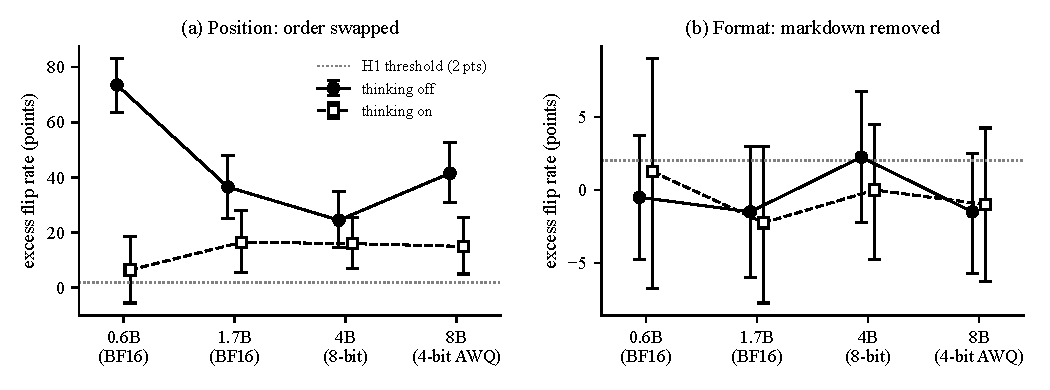
\includegraphics[width=\linewidth]{fig_excess.pdf}
\caption{Excess flip rate (flip rate minus noise floor) with 95\% bootstrap CIs, $n=100$ pairs. Filled circles:
thinking off; open squares: thinking on. Dotted line: 2-point H1 threshold. The x-axis mixes model size with
weight precision. (a) Order swaps change verdicts beyond noise in seven of eight configurations. (b) The
pre-registered format flip measure stays near zero; see Figure~\ref{fig:pref}b for the direct format measure.}
\label{fig:excess}
\end{figure}

\subsection{Format bias (RQ1)}
On the pre-registered measure, removing markdown does not change the winning answer beyond noise. Format excess
flip rates lie between $-2.2$ and $+2.2$ points, and every CI includes zero. These intervals reach up to 9 points,
so they do not rule out effects above the 2-point threshold: \textbf{H1 is not supported for format at $n=100$}.

The direct measure tells a different story (Figure~\ref{fig:pref}b). When exactly one answer keeps its markdown,
four configurations choose that answer significantly more often than 50\% (Holm-adjusted): 1.7B off (54.0\%),
4B off (56.2\%), 4B on (58.0\%) and 8B off (53.5\%). The other four stay within 50.5--52.2\%. Markdown
therefore tilts verdicts, but its effects on stripped winners and stripped losers offset, which hides it from the
flip measure.

\begin{figure}[H]
\centering
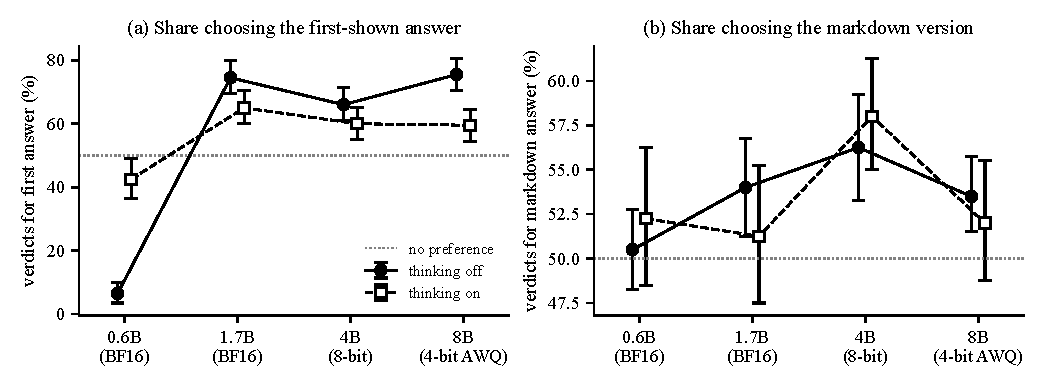
\includegraphics[width=\linewidth]{fig_preference.pdf}
\caption{Direction of the biases, $n=100$ pairs, 95\% bootstrap CIs. The dotted line marks no preference (50\%).
(a) Share of verdicts for the answer shown first. (b) Share of verdicts for the markdown version when only one
answer keeps its markdown.}
\label{fig:pref}
\end{figure}

\subsection{Effects of size and thinking (RQ2)}
\label{sec:h2}
\textbf{Thinking.} The GEE edit$\times$thinking term is negative ($\beta=-1.55$, SE 0.17, $p<0.001$). The AME is
a 30.5-point reduction in excess position flips (bootstrap CI 24.5--37.0). This average is dominated by 0.6B,
whose drop of 67.0 points comes with a large rise in noise. Excluding 0.6B, the reduction is 18.3 points
(GEE $p<0.001$). Per size, the drops are 20.0 points at 1.7B (CI 6.0--34.0), 8.5 points at 4B ($-2.5$ to 19.5)
and 26.5 points at 8B (13.5--39.5). The two modes also use different sampling settings, so these estimates include any effect of the settings
themselves. The proposal's sampling check (thinking off with thinking-mode settings) separates the two and is
scheduled for the full study.

\textbf{Size.} The edit$\times\log_2$size term is not significant ($\beta=-0.06$, SE 0.08, $p=0.47$). The AME is
$-3.6$ points per doubling (CI $-6.3$ to $-0.2$). The AME interval can exclude zero while the logit term does not,
because the AME also reflects how the noise floor changes with size on the probability scale. The pattern is not
monotone: with thinking off, the excess is 73.5, 36.5, 24.5 and 41.5 points from 0.6B to 8B. The interval
contains values on both sides of the 3-point threshold, so neither a size effect nor equivalence to zero is
established. Size is also confounded with precision.

\subsection{Agreement with human voters}
Judge accuracy against the Arena vote is 51--66\% (Cohen's $\kappa$ 0.04--0.34), with Wilson intervals of about
$\pm$10 points. Chance is 50\%. On the same pairs, a length-only rule (the longer answer wins) reaches 57\%
($\kappa=0.14$), and one draw of random verdicts reaches 58\% ($\kappa=0.18$), which illustrates the
$\pm$10-point noise. The configurations cannot be ranked against each other at this sample size. Swap-and-average
agreement, which removes the order effect, ranges from 50.5\% to 64\%. Since voters themselves favour markdown
(Section~\ref{sec:data}), agreement may partly reward format preference.

\subsection{Example}
For the prompt \emph{``Create a sarcastic, meta-style one-liner to promote Deadpool''}, voters preferred
DeepSeek-R1's answer ($a$) over DeepSeek-V3's ($b$). The 1.7B judge without thinking returned \texttt{[[A]]}
(``the first answer'') in all ten calls. It therefore picked $a$ whenever $a$ was shown first and $b$ whenever $b$
was shown first, with or without markdown. Its verdict was decided by order alone.

\section{Discussion}
\label{sec:disc}
\textbf{Hypotheses (interim, $n=100$, mixed precision).}
\begin{itemize}
\item \textbf{H1.} Supported for position: 8B with thinking has an excess of 15.0 points, CI 5.0--25.5.
Not supported for format on the pre-registered flip measure, which is insensitive to a consistent lean. The direct
markdown-preference measure shows a small format lean in four configurations.
\item \textbf{H2.} Thinking reduces position bias by an amount well above the 3-point smallest effect of interest,
but the estimate partly reflects the sampling difference between modes (Section~\ref{sec:h2}). The size effect is
inconclusive and confounded with quantization.
\item \textbf{H3.} Not yet tested; the 500 UltraFeedback brackets are built.
\end{itemize}

Position acts as a strong default, and thinking dampens but does not remove it. Format works differently:
markdown rarely reverses a verdict beyond noise, but it shifts the overall share of verdicts toward the formatted
version. Whether this shift concentrates in close comparisons is untested. Repeated selection could amplify such
a shift, which is what H3 will test.

Our ordering, position bias larger than format bias, is the reverse of \citet{soumik2026judging}. Three
differences may explain this. We use small open judges, which have strong slot defaults. Both answers in our pairs
already use markdown, so we remove only part of the formatting rather than contrasting markdown with prose. And
our format measure uses a 50\% null that cancels content effects. The full study will separate these
explanations by measuring style on the larger pool.

\section{Limitations and Threats to Validity}
\begin{itemize}
\item \textbf{Sample size and multiplicity.} We use 100 of the 1{,}000 planned pairs per pool. Per-configuration
CIs are unadjusted. Five of eight position effects survive Bonferroni adjustment.
\item \textbf{Precision and backend.} 4B is 8-bit and 8B is 4-bit AWQ on a different backend and GPU, whereas the
contract specifies 16-bit weights on one backend. Comparisons across sizes therefore mix model size with
quantization and backend.
\item \textbf{Sampling confound.} The two modes use different model-card sampling settings, and the
sampling check has not yet been run, so the thinking effect includes any effect of the settings.
\item \textbf{Subset composition.} Position bias is measured on markdown-heavy pairs, 84\% of them from 2025, not
on the 2023 position pool. Results by source are in Appendix~\ref{app:robust}; only 16 pairs come from 2023.
\item \textbf{Noise correction.} Subtracting the noise floor assumes that sampling noise and the edit's effect
add. When noise is high (0.6B with thinking), this understates order effects.
\item \textbf{Edit scope.} Only headings, bold and bullets are stripped; italics and numbered lists remain.
\item \textbf{Data and audit provenance.} The 2023 data came from a mirror, and the audit was AI-assisted with
team sign-off pending. Two audit-flagged pairs remain in the subset (sensitivity in Appendix~\ref{app:robust}).
\item \textbf{Human labels.} Voters saw rendered markdown and preferred it.
\end{itemize}

\section{Progress Against the Proposal and Plan}
\label{sec:plan}
\begin{table}[H]
\centering\small
\caption{Status against the proposal's timeline and deviations.}
\label{tab:plan}
\begin{tabularx}{\linewidth}{>{\raggedright\arraybackslash}p{4.2cm} >{\raggedright\arraybackslash}p{2.1cm} X}
\toprule
Proposal item (week) & Status & Deviation and reason \\
\midrule
Data check, frozen pools (W5) & Done & Context-fit filter ($\leq$6{,}000 tokens) and one pair per prompt added. \\
Pilot and frozen evaluation contract (W5) & Done & The contract was frozen after a local pilot; there was no hosted pilot. \\
Harness and preliminary estimates on two sizes (W7) & Done, ahead of plan & All four sizes ran, on 100 pairs. \\
Compute: Kaggle T4, vLLM, FP16 (plan) & Changed & The Kaggle plan was dropped. We used a laptop (MLX) and an 8\,GB GPU (vLLM); 4B and 8B were quantized. OpenRouter and Together do not serve these checkpoints. \\
Sampling-mode check (planned) & Not yet run & Scheduled for the full study (200 pairs per size). \\
Paraphrased-prompt check & Not started & Planned for the full run. \\
Full study, H1--H3 (W9--10) & Not started & Request manifest of 151{,}296 calls is ready. \\
\bottomrule
\end{tabularx}
\end{table}

\textbf{Next steps (weeks 8--10).}
\begin{enumerate}
\item Run the full 1{,}000-pair position and format pools for all four sizes on one 16-bit GPU endpoint, such as
UCSD DSMLP or a rented L4/A100. This removes the precision and backend confounds.
\item Fit the pre-registered GEE (position and format, condition $\times$ size $\times$ thinking, Holm across four
tests) and run the equivalence tests.
\item Complete the sampling-mode check for all sizes and run the paraphrased-prompt check.
\item Test H3 on the 500 UltraFeedback brackets (format drift and selection regret), and compute human agreement
on MT-Bench expert votes.
\item Complete team sign-off of the audit and re-run on the official 2023 file.
\end{enumerate}
If compute runs short, we follow the proposal's order: drop the paraphrase check, then 8B with thinking, then H3.
We never go below 1{,}000 pairs per cell.

\paragraph{Team contributions.} Roles follow the proposal: Member 1, judge harness and logging; Member 2, markdown
stripping and audits; Member 3, data pools and human agreement; Member 4, UltraFeedback bracket; Member 5,
statistics, figures and evaluation contract. \textit{[Team: confirm the name for each role before submission.]}

\paragraph{AI usage disclosure.} We used Claude to help write the data pipeline, the judge harness and the
analysis code, to run the AI-assisted first pass of the stripping audit, and to draft this report. All numbers
are computed by the released scripts from raw judge logs. Audit sign-off by the team is pending.

\begin{thebibliography}{13}\small
\bibitem[Gao et~al.(2023)]{gao2023scaling} L.~Gao, J.~Schulman, J.~Hilton. Scaling laws for reward model
overoptimization. \emph{ICML}, 2023. arXiv:2210.10760.
\bibitem[Huang et~al.(2026)]{huang2026reasoning} H.~Huang, X.~Wu, M.~Yang, Y.~Arase. Reasoning model is superior
LLM-judge, yet suffers from biases. \emph{Workshop on Evaluating Evaluations (EvalEval)}, 2026.
arXiv:2601.03630.
\bibitem[Cui et~al.(2024)]{cui2024ultrafeedback} G.~Cui et~al. UltraFeedback: boosting language models with
scaled AI feedback. \emph{ICML}, 2024. arXiv:2310.01377.
\bibitem[Lin et~al.(2024)]{lin2024awq} J.~Lin et~al. AWQ: activation-aware weight quantization for on-device LLM
compression and acceleration. \emph{MLSys}, 2024. arXiv:2306.00978.
\bibitem[Qwen Team(2025)]{qwen2025qwen3} Qwen Team. Qwen3 technical report. arXiv:2505.09388, 2025; Qwen3-8B
model card, Hugging Face.
\bibitem[Jayarao et~al.(2025)]{jayarao2025explicit} P.~Jayarao, H.~Gupta, N.~Varshney, C.~Dwivedi. Explicit
reasoning makes better judges: a systematic study on accuracy, efficiency, and robustness. arXiv:2509.13332, 2025.
\bibitem[Soumik(2026)]{soumik2026judging} S.~K.~Soumik. Judging the judges: a systematic evaluation of bias
mitigation strategies in LLM-as-a-judge pipelines. arXiv:2604.23178, 2026.
\bibitem[Wang et~al.(2025)]{wang2025assessing} Q.~Wang et~al. Assessing judging bias in large reasoning models:
an empirical study. arXiv:2504.09946, 2025.
\bibitem[Yang et~al.(2026)]{yang2026auditing} Z.~Yang, Y.~Hou, X.~Yang. When the judge changes, so does the
measurement: auditing LLM-as-judge reliability. arXiv:2607.08535, 2026.
\bibitem[Zhang et~al.(2025)]{zhang2025lists} X.~Zhang, W.~Xiong, L.~Chen, T.~Zhou, H.~Huang, T.~Zhang. From lists
to emojis: how format bias affects model alignment. \emph{ACL}, 2025. arXiv:2409.11704.
\bibitem[Zheng et~al.(2023)]{zheng2023judging} L.~Zheng et~al. Judging LLM-as-a-judge with MT-Bench and Chatbot
Arena. \emph{NeurIPS Datasets and Benchmarks}, 2023.
\bibitem[Zhou(2026)]{zhou2026selfplay} C.~Zhou. More convincing, not more correct: self-play reward hacking of
reference-free LLM judges. arXiv:2607.05904, 2026.
\bibitem[Zhou et~al.(2026)]{zhou2026taxonomic} H.~Zhou et~al. Toward robust LLM-based judges: taxonomic bias
evaluation and debiasing optimization. arXiv:2603.08091, 2026.
\end{thebibliography}

\appendix
\section{Robustness}
\label{app:robust}
\begin{table}[H]
\centering\small
\setlength{\tabcolsep}{4pt}
\caption{Robustness of the main results. Position excess without the two audit-flagged pairs ($n=98$); position
excess by source; Bonferroni (8-configuration) 95\% interval; format flips split by whether the stripped answer
was the baseline winner or loser.}
\label{tab:robust}
\begin{tabular}{l r rr r rr}
\toprule
& \multicolumn{1}{c}{$n=98$} & \multicolumn{2}{c}{By source (excess)} & & \multicolumn{2}{c}{Format flip when stripping} \\
\cmidrule(lr){2-2}\cmidrule(lr){3-4}\cmidrule(lr){6-7}
Configuration & Excess & 2023 ($n=16$) & 2025 ($n=84$) & Bonferroni CI & winner & loser \\
\midrule
0.6B, off & 73.0 & 75.0 & 73.2 & [58.5, 86.0] & 13.5 & 12.5 \\
0.6B, on & 5.6 & 21.9 & 3.6 & [$-10.0$, 24.0] & 40.0 & 35.5 \\
1.7B, off & 35.2 & 6.2 & 42.3 & [20.0, 52.9] & 19.0 & 11.0 \\
1.7B, on & 16.3 & 3.1 & 19.0 & [1.0, 32.0] & 20.5 & 18.0 \\
4B 8-bit, off & 24.0 & 9.4 & 27.4 & [10.5, 38.5] & 22.0 & 9.5 \\
4B 8-bit, on & 15.3 & 3.1 & 18.5 & [4.0, 29.0] & 22.0 & 6.0 \\
8B 4-bit, off & 40.3 & 6.2 & 48.2 & [26.0, 56.0] & 11.5 & 4.5 \\
8B 4-bit, on & 15.8 & 9.4 & 16.1 & [1.0, 29.0] & 15.0 & 11.0 \\
\bottomrule
\end{tabular}
\end{table}
Removing the two audit-flagged pairs changes no position excess by more than 1.3 points. Position bias is
concentrated in the 2025 pairs, which are longer and more heavily formatted, but only 16 pairs come from 2023.
The repeated runs used for the noise floor were not copies: identical full outputs occur only for 1 of 200 inputs
(0.6B off) and 21 of 200 (1.7B off), and never in the batched 4B and 8B runs.

\section{Reproducibility}
Code is in \url{src/dsc261/}; notebooks 01--06 produce every table. Frozen data hashes are in
\url{data/processed/freeze_manifest.json}, and raw judge logs are in \url{api/}. All sampling uses seed
261. The report's numbers are regenerated by \url{scripts/report_stats.py} and
\url{scripts/report_extra.py}.
\end{document}
